\begin{CJK}{UTF8}{gkai}
\chapter{数值和编程技术}
\end{CJK}


\begin{CJK}{UTF8}{gbsn}
计算机图形学领域充满了复杂的数学,图形程序通常充满了计算密集型的操作。简化计算的技术和技巧或有用的近似总是受欢迎的。本节包含的Gems为那些喜欢“关注细节”的程序员增加了技巧。


第一个Gem描述了IEEE标准平方根运算的快速近似,并改进了前一个Gem中提出的技术。第二个Gem描述了围绕众所周知的UNIX(tm)内存分配器“malloc()”放置的包装器,以提高其可用性和可预测性。第三个Gem解释了如何考虑由轨道球控制的3-D旋转,并提供了背后的群论数学。第四个Gem简要介绍了区间算法以及如何在计算机图形学中使用它。


第五Gem讨论了与常用的两个、三个或更多数字的循环排列技术相关的效率问题。第六Gem讨论了如何选择颜色来突出显示或选择图像特征,并提出了一个类比魔方的空间!第7个Gem处理的是生成具有各种分布的随机点集,均匀的和其他的。这些技术对于分布射线追踪和其他蒙特卡罗方法非常有用。最后两个Gems采用了二维和三维空间中经常使用的一些概念,并将它们扩展到高维空间中。

\newpage
\section{IEEE 快速平方根}
\begin{center}
\small{
Steve Hill\\
University of Kent\\
Canterbury, Kent, United Kingdom}
\end{center}
这个gem是Paul Lalonde和Robert Dawson在Graphics Gems i中提出的快速平方根算法的重新实现。


在我的实现中,我添加了一个额外的例程,它允许将平方根表转储为C源代码。该文件可以单独编译,以消除在运行时创建表的必要性。


新的例程使用IEEE双精度浮点格式。我包含了许多有用的\#defines ,以使程序更易于访问。注意,在某些体系结构中,单词的顺序是颠倒的。常数MOST\_SIG\_OFFSET 可以设置为1或0,以允许这一事实。


表的大小可以通过改变常量SQRT\_TAB 大小来调整。它一定是4的幂。恒定的MANT\_ SHIFTS必须相应地进行调整——如果将表的大小增加四倍,那么从3MANT\_SHIFTS 中减去2。


See also G1, 403; G1, 424; G2, 387.\\

\section{一个简单的快速内存分配器}
\begin{center}
\small{
Steve Hill\\
University of Kent\\
Canterbury, Kent, United Kingdom}
\end{center}

这个Gem描述了一个简单的内存分配包,可以用来代替传统的malloc()库函数。该包维护一个内存块链表,以顺序的方式从其中分配内存。如果一个块用完,则从下一个块分配内存。如果下一个块是NULL,则使用malloc()分配一个新块。


我们把内存块的列表称为池。一个池可以被全部释放,也可以被重置。在前一种情况下,使用库函数free()将分配给池的所有内存返回给系统。在后一种情况下,不会释放任何内存,但会重置池的高水位标记。这允许在一个操作中丢弃池中分配的所有数据,几乎没有任何开销。然后池中的内存就可以重用了,不需要重新分配。


这个包允许程序员创建多个池,并在它们之间切换。


该方案的一些优点是:



\begin{itemize}
	\item 内存分配很快。


\item 数据可能具有更大的局部性。


\item 我们不再需要每个数据结构都有一个免费的例程。


\item 重置池非常简单。这可能会取代对free()库例程的许多调用。


\item 内存泄漏的可能性较小。

\end{itemize}

主要的缺点是:

\begin{itemize}
  \item 单个结构不能被释放。这可能会导致更大的项目驻留。
\end{itemize}


该软件包已成功用于射线追踪程序。使用了两个池。第一个池保存在读取模型文件时创建的永久数据。第二个池用于在呈现过程中创建的临时数据。在计算完每个像素后重置该池。


该一揽子方案的合并产生了三个重大影响。首先,程序运行得更快。虽然速度不是特别快,但是程序的大部分时间都花在计算十字路口,而不是分配内存上。其次,许多操作的代码变得更简单。这是因为消除了对释放内存的调用。最后,所有的空间泄漏都被根除了。这个程序由许多人共同开发,在某些情况下,对适当的内存分配函数的调用被忘记了。使用包消除了对这些调用的需要;因此,空间泄漏也被消除了。

\newpage
\section{滚动球}

\begin{center}
\small{
Andrew J. Hanson\\
Indiana University\\
Bloomington, Indiana}
\end{center}

交互式图形系统通常需要允许用户使用常用的二维输入设备(如鼠标)在三维空间中自由旋转图形对象的技术。实现这一目标受到一个事实的阻碍,即从输入设备的两个参数到定向的三个参数空间没有单一的自然映射。


在这里,我们介绍了鼠标驱动三维方向控制的滚动球方法,以及它在其他科学可视化问题上的一些有趣的扩展。这种技术利用连续的二维运动(以球在平桌上滚动而不滑动为模型)来达到任意的三维方向。与其他各种方法不同,滚动球方法只有一个状态,并且完全与上下文无关:可以关闭鼠标光标,忽略移动的历史或演进状态,但仍然确切地知道下一个增量鼠标移动将会产生什么效果。对于从直接操作印象中获益的应用程序来说,这个属性非常有吸引力。


很明显,鼠标可以控制围绕两个轴(图1中的$\mathbf{x}$和$\mathbf{y}$方向)的旋转。令人惊讶的是,滚动球还自然地包含了诱导屏幕垂直方向(图1中的$\mathbf{z}$轴)的顺时针和逆时针旋转的能力。根据空间旋转的群体理论的一个基本但违反直觉的性质,在小的顺时针圆周上移动滚动球控制器必然会产生小的逆时针旋转,反之亦然。这就解释了为什么一个明显不可能的三度转动自由度确实可以通过一个上下文无关的二自由度输入设备产生。


\begin{figure}
\centering
	\subfigure[由它们自己渲染的场景中的一簇物体。]{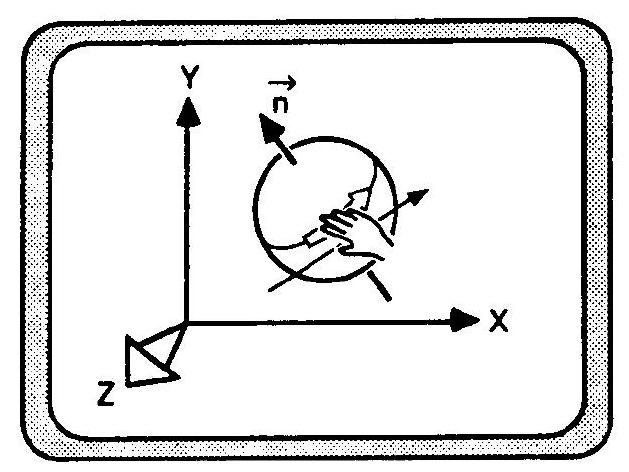
\includegraphics[max width=.35\columnwidth]{2022_11_30_0cbb01a33d99487fc27fg-084}}\hspace{5pt}
	\subfigure[前景和背景物体的合成图像。前景是“聚焦”。]{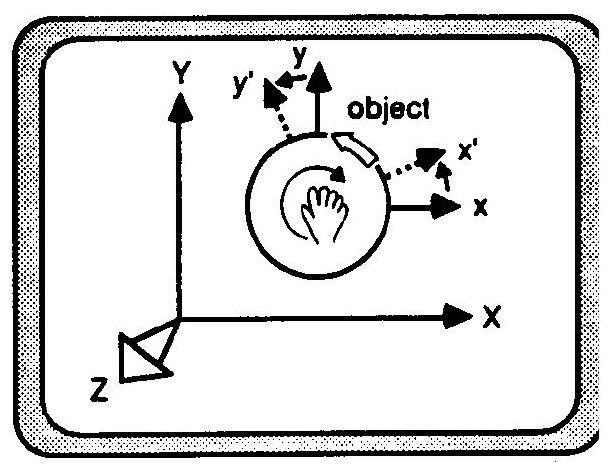
\includegraphics[width=.35\columnwidth]{2022_11_30_0cbb01a33d99487fc27fg-084(1)}}
	\caption{滚动球算法中使用的两种基本技术用于实现图形对象的任意空间旋转。a)用鼠标按黑色箭头指示的方向移动手,使物体绕位于屏幕平面上的轴$\vec{n}$旋转,即使赤道沿空心箭头方向旋转。b)小圈移动手,使物体绕屏幕平面法线旋转,方向与手的运动方向相反,再次旋转赤道沿空心箭头方向。}
\end{figure}

下面给出的滚动球算法的数学形式实际上是Chen等人(1988)在广泛调查方向控制方法中所研究的算法的一部分;我们的方法以Chen等人(1988)没有处理过的方式利用和扩展了算法的属性。滚动球应该被理解为一种新颖的、上下文无关的方法,它利用了通常以上下文相关的方式使用的已知旋转算法。


下面的处理包括两个主要部分。第一部分介绍了如何使用滚动球法进行三维定位控制,以及如何在交互式图形系统中实现它。第二部分描述了如何将滚动球方法扩展到科学可视化中极为重要的其他转换组;滚动球法被看作是一个迷人的工具,在它自己的权利可视化变换组的性质。



\subsection*{使用方法}
为了理解这个方法的基本原理,假设一个球放在桌子上,在你手掌的水平下方。


球绕任何与桌面平行的轴旋转时,都是通过手在垂直于轴的方向上水平移动,从而使球绕该轴旋转。注意,这个类的任何单一运动都不会产生围绕垂直轴的旋转,垂直于手掌的轴。


然而,如果你把你的手平放在一个球的顶部,并在水平的小圆圈中移动你的手,球实际上会绕着垂直轴向相反的方向旋转。


控制空间方向的滚动球算法是通过将要旋转的图形对象的方向作为球本身的方向来实现的,同时使用鼠标(或类似的二维输入设备)来模拟手掌的动作。


通过执行鼠标(或手)的指示动作,可以使用滚动球算法在显示的图形对象上实现以下效果:


\begin{itemize}

\item 绕水平屏幕线或$x$-轴旋转,是通过相对于查看器向前或向后移动鼠标来实现的。


\item 通过向左或向右移动鼠标,可以旋转垂直屏幕线或y轴。


\item 绕屏幕平面上的对角线旋转,我们用向量$\vec{n}$表示其方向,通过垂直移动鼠标到$\vec{n}$来实现,就像手掌在绕轴$\vec{n}$旋转圆柱或球一样。


\item 小的顺时针旋转垂直于屏幕,或z轴,通过移动鼠标在小的,逆时针的圆圈。更明显的旋转是通过使用更大的圆周运动来实现的。


\item 小的逆时针旋转,垂直于屏幕是通过移动鼠标在小的,顺时针的圆圈。


\item 围绕屏幕垂直方向的大旋转是通过向任何方向旋转对象$90^{\circ}$来实现的,围绕原始屏幕垂直轴旋转所需的量(现在位于屏幕平面上),然后旋转$90^{\circ}$来恢复原始屏幕垂直轴的方向。这个动作本质上是一个大的长方形运动,与绕屏幕垂直旋转的小圆形运动形成对比。


\end{itemize}

图1总结了两个最基本的动作,绕屏幕平面上的轴$\vec{n}$旋转和绕屏幕垂直轴旋转。


输入设备光标的位置与滚动球算法无关,在旋转操作期间,它通常对用户是不可见的。计算只需要先前和当前设备位置之间的差异,因此通常需要在每次移动后将鼠标弯曲到屏幕中央,以防止它离开交互窗口。因此,该方法是真正的上下文无关的,非常适合强调直接操作的用户界面。

\subsection*{实现}
滚动球算法是通过取一个给定的增量输入设备运动来定义一个在右屏幕坐标系中包含组件($dx, dy$)的向量来实现的。右旋轴$\vec{n}$被定义为位于屏幕平面上的垂直于输入设备运动的以下单位向量:


\begin{align}
\mathrm{n}_{\mathrm{x}}=\frac{-\mathrm{dy}}{\mathrm{dr}}, \quad \mathrm{n}_{\mathrm{y}}=\frac{+d \mathrm{x}}{\mathrm{dr}}, \quad \mathrm{n}_{\mathrm{z}}=0
\end{align}

这里我们定义了输入设备的位移$d r=\left(\mathrm{dx}^{2}+\mathrm{dy}^{2}\right)^{1 / 2}$。

其次,引入了该算法的单一自由参数——有效滚动半径$R$,它决定了旋转角度对位移$d R$的灵敏度;如果$d r$只有几个像素,那么大约100的$ r$值是合适的。我们选择旋转角度为$\theta=\arctan (\mathrm{dr} / \mathrm{R}) \approx(\mathrm{dr} / \mathrm{R})$,使

\begin{align}
\begin{aligned}
&\cos \theta=\frac{R}{\left(R^{2}+d r^{2}\right)^{1 / 2}} \\
&\sin \theta=\frac{d r}{\left(R^{2}+d r^{2}\right)^{1 / 2}}
\end{aligned}
\end{align}

绕轴$\vec{n}$旋转一个角度$\theta$的矩阵的一般形式是,其中$\vec{n} \cdot \vec{n}=1$,(参见M. Pique在Graphics Gems I, p. 446 [Glassner, 1990]中的“矩阵技术”):

\begin{align}
\left|\begin{array}{ccc}
\cos \theta+\left(n_{x}\right)^{2}(1-\cos \theta) & n_{y} n_{x}(1-\cos \theta)-n_{z} \sin \theta & n_{x} n_{z}(1-\cos \theta)+n_{y} \sin \theta \\
n_{y} n_{x}(1-\cos \theta)+n_{z} \sin \theta & \cos \theta+\left(n_{y}\right)^{2}(1-\cos \theta) & n_{y} n_{z}(1-\cos \theta)-n_{x} \sin \theta \\
n_{z} n_{x}(1-\cos \theta)-n_{y} \sin \theta & n_{z} n_{y}(1-\cos \theta)+n_{x} \sin \theta & \cos \theta+\left(n_{z}\right)^{2}(1-\cos \theta)
\end{array}\right|
\end{align}


将Eq.(2.3.1)中$\vec{n}$的值代入Eq.(2.3.3),得到滚动球旋转矩阵

\begin{align}
\left|\begin{array}{ccc}
\cos \theta+(d y / d r)^{2}(1-\cos \theta) & -(d x / d r)(d y / d r)(1-\cos \theta) & +(d x / d r) \sin \theta \\
-(d x / d r)(d y / d r)(1-\cos \theta) & \cos \theta+(d y / d r)^{2}(1-\cos \theta) & +(d y / d r) \sin \theta \\
-(d x / d r) \sin \theta & -(d y / d r) \sin \theta & \cos \theta
\end{array}\right|
\end{align}



其中三角函数的值由式(2.3.2)给出。我们观察到:

\begin{itemize}
\item 在应用式(2.3.4)之前,必须将所有向量转换到所需的旋转中心。


\item 旋转必须在一个单独的步骤中执行,如Eq.(2.3.4)。执行旋转作为一个序列,例如,首先绕$x$-轴,然后绕y轴,将给出一个完全不同的结果(尽管,由于微妙的原因,差异可能几乎是不可观察的)。


\item 更改$\vec{n}$的整体符号将产生围绕对象的视点旋转,而不是视图内的对象旋转。小的顺时针的手运动将产生小的顺时针旋转的视点,但在视图中心的对象将继续逆时针旋转。这一现象源于群理论对身体固定旋转和空间固定旋转描述的符号差异(Whittaker, 1944)。

\end{itemize}

\subsection*{滚球法的推广}
当我们分析滚动球法的群论背景时,各种相关的应用立即浮现出来。在这里,我们总结了普通旋转所涉及的基本群论,以及几个易于实现的扩展。这些技术对于许多科学可视化应用程序都很有用,包括建立关于一般群体的直觉。如果读者对群论没有兴趣,只是想知道如何实现和使用算法,就不必再读下去了。

\subsection*{无穷小旋转的群论}
涉及滚动球行为的基本群论(Edmonds, 1957)可以总结如下:如果我们定义$L_{i}, i=\{x, y, z\}$为旋转群$O$(3)的无穷小产生子,具有正旋转的右手约定,那么我们就有了对易关系

\begin{align}
\left[\mathrm{L}_y, \mathrm{L}_{\mathrm{z}}\right]=-\mathrm{L}_x, \\
\left[\mathrm{L}_z, \mathrm{L}_{\mathrm{x}}\right]=-\mathrm{L}_y, \\
\left[\mathrm{L}_x, \mathrm{L}_{\mathrm{y}}\right]=-\mathrm{L}_z,
\end{align}
其中我们使用了定义$[\mathrm{A}, \mathrm{B}]=\mathrm{AB}-\mathrm{BA}$。这些无穷小生成器可以表示为矩阵,也可以表示为这种形式的微分算子


$$
\mathrm{L}_{\mathrm{x}}=\mathrm{y} \frac{\partial}{\partial \mathrm{z}}-\mathrm{z} \frac{\partial}{\partial \mathrm{y}}
$$

和它的循环排列。方程式中的负号。(5-7)不是任意的,而是由我们的惯例决定的,$\mathrm{L}_{\mathrm{i}}$使用右手规则绕第i轴旋转一个向量。这个负号直接导致了观测到的反旋转,是旋转群性质的必然结果。


\subsection*{四元数旋转,$2 \times 2$矩阵,和SU(2)旋量}
滚动球变换用于定义四元数旋转(例如,参见Shoemake, 1985,或p - g的“使用四元数”)。Maillot在Graphics Gems I,第498页[Glassner, 1990])甚至比普通的空间旋转更自然。这是因为四元数公式等价于组SU(2)的更标准的$2 \times 2$矩阵表示法,SU(2)是通常旋转组O(3)的双重覆盖(Edmonds, 1957)。(尽管这两个基团对应完全不同的拓扑空间,但它们被滚动的球利用的无穷小性质是相同的。)


为了利用滚动球进行SU(2)转动,我们用

\begin{align}
\mathrm{U}=I_{2} \cos \frac{\theta}{2}-i\vec{n} \cdot \vec{\sigma} \sin \frac{\theta}{2},
\end{align}
其中$I_{2}$是$2 \times 2$单位矩阵,$\vec{\sigma}$表示SU(2)服从循环关系$\sigma_x^{2}=1, \sigma_x \sigma_Y=i \sigma_z$的$2 \times 2$矩阵基。这相当于一个基于四元数的转换,其中$(c, u)=(\cos (\theta / 2)$, $\vec{n} \sin (\theta / 2)$)。注意,与完整矩阵Eq.(3)相比,Eq.(8)合并滚动球的基本参数要简单得多。

更改$\vec{n}$的整体符号将产生围绕对象的视点旋转,而不是视图内的对象旋转。


矩阵Eq.(8)的元素可以根据需要从Eq.(3)中计算一个普通的矢量旋转矩阵,也可以直接用作$2 \times 2$矩阵来旋转旋量(Edmonds, 1957),这是旋转群所能作用的最基本对象。

\subsection*{欧几里得四维}
在四维欧氏空间中,0(4)群有6个转动自由度,而不是由于$0(3)$而在三维空间中存在的3个。


6个$0(4)$旋转算子$\mathrm{L}_{\mu v}, \mu, v=\{1,2,3,4\}, L_{\mu v}=-L_{\mu v}$,可以通过定义以下组合分解为$O (3) \times 0 (3)$:

\begin{align}
L_{\mathrm{i}}^{\pm}=\frac{1}{2}\left(\frac{1}{2} \epsilon_{\mathrm{ijk}} L_{\mathrm{jk}} \pm L_{4 \mathrm{i}}\right) .
\end{align}
这里$\epsilon_{i j k}$是三维中的完全反对称张量,我们使用重复罗马指标从1到3求和的惯例。每一个组合都服从独立的$0(3)$变换关系,

\begin{align}
\left[L_{1}^{\pm}, L_{\mathrm{j}}^{\pm}\right]=-\epsilon_{\mathrm{ijk}} L_{\mathrm{k}}^{\pm}, \quad\left[L_{\mathrm{i}}^{\pm}, L_{\mathrm{j}}^{\mp}\right]=0,
\end{align}
因此可以使用$O(3)$滚动球算法单独控制。以这种方式产生的旋转可以写成

\begin{align}
R^{\pm}=I_{4} \cos \theta+\vec{n}  \cdot \vec{L}^{\pm} \sin \theta,
\end{align}


其中

$$
\vec{n} \cdot \vec{L} \pm=\left|\begin{array}{cccc}
0 & -n_{z} & n_{y} & \mp n_{x} \\
n_{z} & 0 & -n_{x} & \mp n_{y} \\
-n_{y} & n_{x} & 0 & \mp n_{z} \\
\pm n_{x} & \pm n_{y} & \pm n_{z} & 0
\end{array}\right|,
$$
单位向量$\vec{n}$通常由式(1)定义。因此,我们可以使用滚动球的两个副本来操纵四维方向的所有自由度,一个为$\mathrm{L}_{1}^{+}$,一个为$\mathrm{L}_{\mathrm{i}}^{-}$。


另一种方法也适用于N维欧氏空间中的旋转,它是将群$O(4)$(或$\mathrm{N}$中的$O(\mathrm{~N}$))分解为$O$(3)子群,并将每个子群视为独立的滚动球变换。

\subsection*{洛伦兹变换}
研究高速物理系统必须使用时空洛伦兹变换,而不是欧几里得旋转。洛伦兹变换将空间和时间混合在一起,保留了一个具有一个负分量的闵可夫斯基空间二次型。纯粹的速度变化,或“加速”,在形式上类似于用双曲函数取代三角函数的旋转。速度$\vec{v}=\hat{} v \tanh \xi$通过矩阵转换向量$(\vec{x},t)$
\begin{align}
\left|\begin{array}{cc}
\delta_{i j}+\hat{v}_{i} \hat{v}_{j}(\cosh \xi-1) & \hat{v}_{j} \sinh \xi \\
\hat{v}_{i} \sinh \xi & \cosh \xi
\end{array}\right| .
\end{align}

为了实现$O(2,1)$洛伦兹转换(它保留了diag $(1,1,-1)$的形式),我们将鼠标运动解释为“洛伦兹滚动球”在鼠标移动方向上的微小速度变化。(我们也可以研究物理时空的变换群$0(3,1)$;不幸的是,导致式(10)的论点的类比需要引入复向量。)


$\mathrm{O}(2,1)$转换的无穷小生成器是boost操作符


$$
B_{\mathrm{x}}=t \frac{\partial}{\partial x}+x \frac{\partial}{\partial t}, \quad B_{y}=t \frac{\partial}{\partial y}+\mathrm{y} \frac{\partial}{\partial t} ,
$$
和操作符

$$
L=x \frac{\partial}{\partial y}-y \frac{\partial}{\partial x}
$$

在$x-y$面上产生旋转。boost算子在旋转下变换为普通向量,$\left[L, B_{x}\right]=-B_{y},\left[L, B_{y}\right]=+B_{x}$,而它们的相互交换产生的旋转符号与类似的$O(3)$算子,$\left[B_{x}, B_{y}\right]=+L$相反。


我们将鼠标输入与$O(2,1)$转换Eq.(12)关联起来,将Eq.(1)替换为

\begin{align}
\hat{v}_x=\frac{+dx}{dr}, \quad \hat{v}_y=\frac{+dy}{dr}
\end{align}

选择boost参数为$\xi=\tanh ^{-1}(\mathrm{dr} / \mathrm{s}) \approx(\mathrm{dr} / \mathrm{s})$,其中's是一个合适的缩放因子,确保$(\mathrm{dr} / \mathrm{s})<1$。


然后我们发现,在小的顺时针方向移动输入设备会产生顺时针方向坐标框架的空间部分的旋转,这与标准$O(3)$旋转的结果相反!这种效应被称为托马斯进动,使滚动球技术成为洛伦兹变换的一种非常自然的技术。


\subsection*{总结}
总之,滚动球技术提供了一种在交互式图形系统中使用二维输入设备控制三个转动自由度的方法,这种方法不依赖于输入设备的状态、位置或历史。由于算法丰富的群论起源,许多相关的科学可视化应用自然而然地出现了。要想熟练使用该技术,用户需要付出一些努力。但是,一旦掌握了这种方法,就会提供与情境无关的、探索性的方向调整,强烈支持直接操作的感觉。

\subsection*{鸣谢}
这项工作的一部分得到了美国国家科学基金会的资助。是- 8511751。

See also G1, 462 .\\

\newpage
\section{区间运算}
\begin{center}
\small{
Jon Rokne\\
The University of Calgary\\
Calgary, Alberta, Canada}
\end{center}


在计算机图形学中,离散化问题发生在两个不同的领域:

\begin{itemize}
\item 计算的最终输出是用有限分辨率的设备显示或打印的二维图像,这会造成诸如混叠等不良影响。


\item 确定位置、强度和颜色所需的计算在通用计算设备或专用图形计算机中进行。在任何一种情况下,存储实数的基本方法都是所谓的浮点表示。这种表示为存储浮点数分配固定数目的二进制位数,浮点数可以是输入或输出量,也可以是中间计算的结果。

\end{itemize}

我们将讨论一种工具,区间分析,它使用有保证的上界和下界来估计和控制在数值计算中可能出现的数值误差,特别是在计算机图形问题中出现的数值误差。区间算术是一门涉及面很广的学科,我们只涉及到一些基本思想。然而,我们注意到区间算术和分析已经导致了基于包含和收缩的新技术的发展,这些技术适用于计算机图形学中的一些问题。


我们首先给出一个可能发生在图形应用程序中的问题的例子。一个基本例程可能包括确定两条线(为了简单起见,在$E^{2}$中)是否平行(也就是说,它们是否有一个有限的交集)。如果它们相交,计算交点。让线条保持原样


\begin{align}
0.000100 x+1.00 y&=1.00 \\
1.00 x+1.00 y&=2.00
\end{align}
假设这个算法是一个三位数四舍五入的算法。四舍五入到五位数的真正解是$x=1.0001$和$y=0.99990$,而使用Forsythe和Moler(1967)中描述的过程,三位数的算术给出$y=1.00, x=0.00$。在本文中,使用不同的计算顺序安排也得到了其他错误的结果。从这个例子可以看出,这样的计算可能有很大的误差,以致于一个应该在区域内的交集实际上可能被计算在区域外。

另一个例子是区域填充,其中区域的连通性依赖于一个计算,该计算可能以与交叉计算相同的方式充满错误。

这样的错误很难防范,最终它们会在计算机生成的场景中产生不受欢迎的工件,并且很难在大型程序中跟踪和纠正。

其中许多误差可以使用区间算法自动控制。它使程序能够给出项目$p$和集合$P$的三个答案之一。


\begin{enumerate}
	\item $p$肯定在$P$中。


\item $p$肯定不在$P$中。


\item 在执行的计算和可用的精度中,不可能告诉$p \in P $或$p \notin P $,也就是说,结果是不确定的。
\end{enumerate}

根据前面的例子,我们可以说直线相交,它们不相交,或者它们是否相交是不确定的。类似地,我们可以声明一个域是连接的,它是没有连接的,或者域是否连接是不确定的。在每一种情况下,可以将决策程序内置于程序中以处理这三种情况。


区间运算有着悠久的历史;然而,它的现代使用源于摩尔(1966)的《区间分析》一书的出版。后来,有大量的出版物专门讨论这个问题。Garloff出版了参考书目(1985,1987),举行了一些会议,最近出版了一份新的苏联期刊,《区间计算》(新技术研究所,1991),完全致力于区间分析。

区间算术定义如下:设 $I=\{A: A=[a, b], a \cdot b$ $\in \mathrm{R}\}$为实紧区间集,设$A, B \in I$。然后区间算术运算定义为

$$
\mathrm{A} * \mathrm{~B}=\{\alpha * \beta: \alpha \in \mathrm{A}, \beta \in \mathrm{B}\} \text {, }
$$
其中 $* \in\{+,-, \cdot, /\}$(注意 / 在 $0 \in B$ 时未定义),即 $A * B$ 的区间结果包含所有可能的点结果 $\alpha * \beta$,其中 $\alpha$ 和 $\beta$ 是实数,使得 $\alpha \in A$ 和 $b\eta in B$ 和 $*$ 是基本的算术运算之一。

这个定义是由下面的论证驱动的。给定两个区间$A$和$B$,我们知道它们分别包含精确的值$x$和$y$。然后定义保证$x * y \in A * B$中用于上述任何操作,即使我们不知道$x$和$y$的确切值。

这个定义在实际计算中不是很方便。令$A=[a, b]$,且$ B=[c, d]$,可得其等价于

\begin{align}
\begin{aligned}
{[a, b]+[c, d]}  &=[a+c, b+d], \\
[a, b]-[c, d]  &=[a-d, b-c], \\
[a, b] \cdot [c, d] &=[\min (a c, a d, b c, b d), \max (a c, a d, b c, b d)], \\
[a, b]/[c, d]  &=[a, b][1 / d, 1 / c] \text { if } 0 \sim[c, d],
\end{aligned}
\end{align}

这意味着在$* \in\{+,-, \cdot, /\}$中的每个区间操作都被简化为真正的操作和比较。


区间算术的一个重要性质是


\begin{align}
\begin{aligned}
A, B, C, D \in A \subseteq B, C \subseteq D, \Rightarrow A_{\sqcup} * C C_{\sqcup} \subseteq B_{\sqcup} & * D \\
& \text { for } * \in\{+,-, \cdot, /\}
\end{aligned}
\end{align}

如果定义了操作。换句话说,如果$A$和$C$分别是$B$和$D$的子集,那么$A * C$是用于任何基本算术操作的$B * D$的子集。因此,在计算的任何阶段引入的错误,如浮点错误或输入错误,都可以被解释。由于式(4)的重要性,它被称为区间运算的包含等度。

如果定义了操作。换句话说,如果$A$和$C$分别是$B$和$D$的子集,那么$A * C$是用于任何基本算术操作的$B * D$的子集。因此,在计算的任何阶段引入的错误,如浮点错误或输入错误,都可以被解释。由于式(4)的重要性,它被称为区间运算的包含等度。

这样做的一个结果是,任何可编程的实计算都可以使用操作之间的自然对应关系嵌入到区间计算中,因此,如果$x \in X \in I$中,则$f(x) \in f(X)$中,其中$f(X)$被解释为$f(. x)$ , $x$替换为$X$,操作替换为区间操作。

间隔算术的另一个重要原理是,它可以在浮点计算机上实现,这样得到的间隔包含使用等式进行的真实间隔计算的结果。(3)和定向四舍五入。有几种软件系统可用于此目的,如PASCAL-SC (Bohlender et al., 1981)。实现只需要注意间隔端点的每个计算都是从间隔的内部向外舍入。

区间算术也有一些缺点:


\begin{itemize}
\item 减法和除法不是加法和乘法的逆运算。

\item 分配律不成立。只有子分配律$\mathrm{a}(\mathrm{B}+$ C) $\subseteq \mathrm{AB}+\mathrm{AC}, \mathrm{a}, \mathrm{B}, \mathrm{C} \in\mathrm{I}$是有效的。

\item 区间算术操作比相应的实际操作大约耗时3倍(尽管某些问题的区间算术实现可能比相应的实际版本运行得更快;参见suffn and Fackerell, 1991)。
	


\end{itemize}

作为使用区间计算的一个简单例子,我们使用三位区间算术来考虑上面给出的相交线问题。根据克拉默法则,我们得到


$$
\mathrm{x}=\left|\begin{array}{cc}
1.00 & 0.000100 \\
2.00 & 1.00
\end{array}\right| /\left|\begin{array}{cc}
0.000100 & 1.00 \\
1.00 & 1.00
\end{array}\right|
$$
和
$$
\mathrm{y}=\left| \begin{array}{cc}
0.000100 & 1.00 \\
1.00 & 2.00
\end{array}\right| / \left|\begin{array}{cc}
0.000100 & 1.00 \\
1.00 & 1.00
\end{array}\right|.
$$
利用区间算法得到
$$
\mathrm{x} \in \mathrm{X}=[0.980,1.03]
$$
和
$$
\mathrm{y} \in \mathrm{Y}=[0.989,1.02],
$$
在每种情况下都包含精确解。这个计算与Forsythe和Moler(1967)引用的计算相比,在实际算术中对应更稳定的计算。如果这个特定的计算序列是在区间算术中执行的,那么间隔会更大,但在所有情况下,准确的结果都包含在结果的区间中。

区间算术的一个有趣的特点是,它可以用来开发新的算法,而不是简单地扩展实际算术中的算法。其中一个例子是摩尔(1966)首先提出的区间牛顿法。假设给定$\mathrm{F}(\mathrm{x})$,并假设我们想要找到在给定区间$X_{0}$中$F(\xi)=0$的点$\xi$。然后定义区间牛顿法为迭代

$$
\mathrm{X}_{\mathrm{n}+1}=\mathrm{m}\left(\mathrm{X}_{\mathrm{n}}\right)-\mathrm{F}\left(\mathrm{X}_{\mathrm{n}}\right) / F^{\prime}\left(\mathrm{m}\left(\mathrm{X}_{\mathrm{n}}\right)\right), \quad \mathrm{n}=0,1, \ldots,
$$
其中$m([a ; b])=\left((a+b) / 2\right.$和$F^{\prime}(X)$是$F$的导数的区间求值。这个方法有一些有趣的性质。

\begin{enumerate}
\item 如果$F$的0 $\xi$存在于$X_{0^{\prime}}$中,则对于所有$n$, $\xi \in X_{n}$中;见Moore(1966)。这意味着初始$X_{0}$中的所有零都保留在后续的间隔中。

\item 如果$X_{n^{\prime}}$对于某个$n$是空的,那么$F$在$X$中没有零(Moore, 1966)。

\end{enumerate}

方程解的区间迭代的进一步性质可以在neuaier(1990)中找到。

该方法可应用于计算机图形学中的射线跟踪。隐式曲面和射线之间的交点计算会导致一个问题,即找到函数$\mathrm{F}(\mathrm{x})=0$的一个(最小)根或所有根(见Hanrahan, 1989)。通过使用区间算术技术,可以保证结果包含在生成的区间中,避免渲染过程中的异常(参见Kalra和Barr, 1989,关于该问题的讨论)。

在Mudur和Koparkar(1984)以及summern和Fackerell(1991)中,我们发现了在隐式表面绘制中使用区间算法,在轮廓绘制算法和面度估计中使用区间算法的进一步讨论,其中它与细分技术相结合,以改善结果。

See also G2, 394.


\newpage
\section{快速生成循环序列}
\begin{center}
\small{
Alan W. Paeth\\
NeuralWare Incorporated\\
Pittsburgh, Pennsylvania}
\end{center}

自由运行的内部循环通常需要一系列重复每个$N$步骤的值或条件。例如,高速z -缓冲区绘制技术(Booth et al., 1986)必须以三个周期执行缓冲区交换和内务管理。当$N$不是2的幂时,直接检查寄存器的低阶位可能不会被用来形成N的计数模。类似地,一个快速的二维N-gon生成器需要循环生成$N$的值序列,顶点$N$与顶点0相同。这个Gem考虑了$N<8$的紧凑方法,它使用的机器指令不超过三条,也不超过三个寄存器。不使用条件逻辑,使得该技术非常适合手工编码。

\subsection*{$\mathbf{N=2}$ (Review)}
我们熟悉的双重“toggle”在true和false之间交替:


\begin{align}
\begin{aligned}
&\text { condition := \textbf{not} (condition); } \quad \textit { True in alternating cases } \\
&\text { \textbf{if} (condition) } . . .
\end{aligned}
\end{align}

类似地,值的双重“循环”是一个简单的交替。当两个值都是预先确定的,一条指令和一个整数寄存器就足够了:



$$
\begin{array}{ll}
\text { \textbf{register}  } a:=v 1 ; & \text { initialize } \\
\text { \textbf{constant}  } c:=v 1+v 2 ; & \\
\text { \textbf{ repeat} } & \textit { cycle } \\
%\quad a:=a-c ; & a:[v 1 \text { v2ن } \cdots]
\qquad a:=a-c ; & a:[v 1 \text { v2} \cdots]
\end{array}
$$

例如,Wirth(1973)通过使用(2.2)来加速质数筛选,生成序列$\left[\begin{array}{lllll}2 & 4 & 2 & 4 & \cdots \end{array} \right]$,该序列表示不能被3除的连续奇数之间的距离(Knuth, 1981)。用逻辑异或操作重写(2.2)的算术,可以得到一种著名的专利方法,以交替的方式反转帧缓冲区的像素。以算术形式,重新推导出适合于灰度帧缓冲区的像素反演方案(Newman和Sproull, 1979)。

通常情况下,循环序列只在运行时指定。对于$N=2$,循环是交换,很容易在三个算术或逻辑操作中完成,而不需要借助第三个持有寄存器,分别在Paeth(1990)和Wyvill(1990)之前的Gems中描述过。

\subsection*{$\mathbf{ N=3}$ (扩展)}
成对交换技术不能优雅地扩展:序列[a, b, c]的循环排列通过交换(例如)位置$(1,2)$和$(2,3)$的元素需要6条指令和3个寄存器。第一性原理循环队列方法需要$\mathrm{N}+1$个寄存器和$\mathrm{N}+1$个赋值。后者虽然简单明了,但仍然超出了序言中规定的指令和寄存器的限制:

$$
\begin{aligned}
& \text { r1 :=r1  \textbf{xor} r2; } \quad \text { r2 :=r2 \textbf{xor} r1; } \quad  &rx :=r 1 ; \quad r 1:=r 2 \text {; } \\
& \text { r1 :=r1 \textbf{xor} r2; } \quad \text { r2:=r2 \textbf{xor} r3; <versus>} \quad &r2:=r 3 ; \quad r 3:=r x ; \\
& \text { r3 := r3 \textbf{xor} r2; } \quad \text { r2 }:=\text { r2 \textbf{xor} r3 }
\end{aligned}
$$
通常,如(2.1)所示,只需要值来触发1-in-N事件。对于$N=3$,两个寄存器和两行就足够了。每个寄存器指令都是紧凑的双运算形式$\ll r x=rx \quad op \quad ry \gg$


$$
\begin{aligned}
& \textbf { register } r1 :=0 ;  &\textit{Three fold trigger } \\
& \textbf { register } r2 :=1;  \\
& \text { \textbf{ repeat}}         & \textit{ cycle: }\\
&\qquad \text { r1 :=r1  \textbf{xor} r2;} &r1:[1\quad 1 \quad 0\quad \cdots] \\
&\qquad \text { r2 :=r2 \textbf{xor} r1; } &r2:[0\quad 1 \quad 1\quad \cdots] 
\end{aligned}
$$

这就产生了所示的三级($r1,r2$)列集。当一个寄存器为零时,就会触发。在假设硬件条件代码是由前面的逻辑操作设置的情况下,对r2的测试简化了操作。测试的阶段可以通过在初始化( $r1, r2)$时替换第三列以外的列来调整。触发2-3次定义了互补集:非零的测试被替换。三个相位不同的1-in-3测试可以同时进行,形成一个循环的开关。


$$
\begin{array}{ll}
\textbf { if } r=0 \textbf { then } \cdots & 1 \text {-in-3, phase }=0 \\
\textbf { if } r1=r 2 \textbf { then } \cdots & 1 \text {-in-3, phase }=1 \\
\textbf { if } r1=0 \textbf { then } \cdots & 1 \text {-in-3, phase }=2
\end{array}
$$

条件和相关块可以嵌入到异或操作中,以利用隐式条件代码感知。也就是说,隐式定义模数为3的计数器的两条异或线不必相邻。

三个寄存器中三个变量的循环排列可以在最少的指令数(3条)内完成。推导过程并不明显,并与后面描述的三重算术情形相关。


\IncMargin{1em}
\begin{algorithm} 
\SetKwData{Left}{left}
\SetKwData{This}{this}
\SetKwData{Up}{up} 
\SetKwFunction{Union}{Union}
\SetKwFunction{WritePixel}{WritePixel}
\SetKwFunction{FindCompress}{FindCompress} 
\SetKwFunction{Register}{register} 
\SetKwFunction{Repeat}{repeat} 
\SetKwFunction{Constant}{constant} 
\SetKwFunction{Xor}{xor} 
\SetKwInOut{Input}{input}
\SetKwInOut{Output}{output}

\SetKwData{EdgeSet}{EdgeSet}
\SetKwData{Point}{point}

	  \Register int  a=c1; \tcp{ Three fold cycle } 
 \Register int  b=c1 \Xor c2 \;
 \Constant int  c=c1 \Xor c2 \Xor c3 \;
 \Repeat \tcp{cycle:}  
 a=a \Xor b;  \tcp{\text{ a: [c1 c2 c3...] }}
 b=b \Xor c \; 
 b=b \Xor a \;
 	 \end{algorithm}
\DecMargin{1em} 
逻辑\textbf{xor}的使用是有价值的,因为元素可以是整数、指针和浮点数的混合序列;算术运算不允许这样做。注意,最后两行都更新了b中的值,而寄存器c从未被写入。这暗示了另一条路线:
$$
\mathrm{b}:=\mathrm{b} \text { \textbf{xor} (a \textbf{xor} } \mathrm{c} \text { ) }
$$
其中$\mathrm{c}$等于一个预先确定的编译时间常数。但是,该值在运行时通常必须占用第三个寄存器。(请参阅c代码中产生循环[1,2,3]的双寄存器变体。)
当只需要触发时,修复$\mathrm{c}=0$将省略循环的中线,重新构造$\mathrm{N}=3$触发情况。另外,这两行可以看作是熟悉的异或交换代码的前两行。因为后者的最后一行与第一行匹配,所以三次通过两行异或代码在两个寄存器上产生的顺序动作与两次通过三行代码产生的顺序动作相同(这是通过指令分组在式(3.1a)中提出的)。两者都定义了恢复双交换:对两个元素进行不少于6步的标识操作。因此,两行代码形成长度为3的循环,同时生成序列$[\mathrm{r} 1, \mathrm{r} 1 \oplus \mathrm{r} 2, \mathrm{r} 2]$。


\subsection*{$\mathbf{N=3,4,6}$}
值得注意的是,长度不超过$N=6$的循环只需要两个寄存器。显然,没有足够的存储空间来交换所有元素,否则$N+1个$寄存器和$N+1个$赋值就足够了。相反,目标是派生一组值(在一个或两个寄存器上),其中所有生成的值都是不同的。因此,寄存器必须“计数”,并与第一性原理代码相竞争,例如快速六边形绘制例程:

$$
\begin{aligned}
&\text{Xval =X\_Value\_Table[(i := (i +1 \textbf{mod} 6))];} \\
&\text{Yval = Y\_Value\_Table[i];}
\end{aligned}
$$
在这里,模数是一个主要的费用:它的成本与整数除法相当。另一种第一性原理方法使用条件逻辑重新启动一个递减的计数器,在现代流水线硬件上产生很大的分支惩罚,而小N则使情况变得更糟。

在(6.2)中可以看到,二维六边形的顶点生成可以使用这样的六重循环:

$$
\begin{aligned}
&\text { \textbf{register} } \mathrm{x}=\mathrm{y}=1 \text {; } \\
&\text { \textbf{repeat} }\\
&\qquad \text {Xval = X\_coord[x :=x+y] ;}\\
&\qquad \text {Yval = Y\_coord[y := y+\textbf{not}(x)]}
\end{aligned}
$$
其中$\bf{not}(\mathrm{x})$是位反转,即$\bf{not}(\mathrm{x})=x \quad \bf{xor} (-1)$在两个互补硬件下。长度为7的数组需要有合适的偏移量,如配套的C代码所示。


\subsection*{$\mathbf{N=6}$ 推导}
非均匀旋转可以用函数组合来模拟。即$F(F\cdots(F([x]))\cdots)=[x]$在不少于$N$步骤。例如,线性分数函数$F(x)=\left[2 x-1\right] /[x+1]$得到$F^{6}(x)=x$ (Yale, 1975)。这种形式可以直接等同于$2 \times 2$矩阵的代数(Birkhoff and MacLane, 1965);为了便于推导,优先处理前者。

两个寄存器的值可以用整数点阵上的点$[x, y]$表示,每个寄存器一个坐标。作为一个(列)向量$v$,函数$F$是一个$2 \times 2$矩阵,它的前乘是$v$。对于给定的$N$, F必须确定为:$\mathrm{F}^{\mathrm{N}} v=\mathrm{I}$。当$\mathrm{F}$是一个剪切矩阵时,旋转可以在三个剪切中实现(Paeth, 1986),每个剪切只需要一个赋值语句(第182页)。当非对角矩阵元素为$\{\pm 1\}$时,不会发生乘法运算,一条机器指令就足够了。全有理形式也产生旋转,但圆周点的集合不是单位根(在复笛卡尔平面上单位圆内刻的$n$边形的顶点)。唯一的解决方案是四次旋转。这种分解是:

$$
\begin{bmatrix}
0 & -1 \\
1 & 0
\end{bmatrix}
=\begin{bmatrix}
1 & 1 \\
0 & 1
\end{bmatrix}
\begin{bmatrix}
 1 & 0 \\
  -1 & 1
\end{bmatrix}
\begin{bmatrix}
1 & 1 \\
0 & 1
\end{bmatrix}.
$$
第一个和第三个矩阵的重新分组(第192页)允许两行旋转,在提供隐式乘2的机器上很有用:


\begin{align}
\begin{aligned}
& \mathrm{x}:=\mathrm{x}+\mathrm{y} ; \qquad \qquad \qquad \mathrm{x}:=\mathrm{x}+\left(2^{*} \mathrm{y}\right) ; \\
& \mathrm{y}:=\mathrm{y}-\mathrm{x} ; \quad < \mathrm{or}>\quad \mathrm{y}:=\mathrm{y}=\mathrm{x} ; \\
& \mathrm{x}:=\mathrm{x}+\mathrm{y} \text {; }
\end{aligned}
\tag{4.1}
\end{align}

这种顺序形式比紧凑的$\{x=-y, y=x\}$形式稍微昂贵一些,当寄存器值可以同时重赋时,就像在硬件中一样。3和6的旋转可以通过寻找符号形式的$\mathrm{X}$和$\mathrm{Y}$剪切的乘积的特征值并将它们与单位根相等来形成,从而确定两个离轴元素的值。在其最紧凑的形式中,这将产生二次方程$z=\frac{1}{2}\left(m \pm \sqrt{m^{2}-4}\right)$,它可以表示$N=\{1,2,3,4,6\}$的单位根$z^{N}=1$,其值分别为$m=\{2,2,1,1,0,1 \}$。使用MAPLE对矩阵方程$(\mathrm{XY})^{\mathrm{N}}=\mathrm{I}$的符号矩阵元素的解,不揭示与下面通解明显不同的实值积分形式:


$$
\begin{aligned}
\left(\begin{bmatrix}
 1 & 0\\
 m\mp2 & \pm 1
\end{bmatrix}\begin{bmatrix}
\mp 1 & 1\\
0 & 1
\end{bmatrix}=\begin{bmatrix}
\pm1 & 1 \\
\pm m-2 & m\mp 1
\end{bmatrix}\right)^N=\begin{bmatrix}
1 & 0\\
0 &1
\end{bmatrix},\\
(\mathrm{m}, \mathrm{N})=\{(-1,3),(0,4),(1,6)\}
\end{aligned}
$$
因此,使用单位元件可以进行三倍和六倍的旋转。考虑到$\cos 60^{\circ}$的不合理性,这是意料之外的。简化的双剪切旋转形式的变形已成为固定顶点到积分位置的优点。注意$\mathrm{N}=(3,4,6\}$的三个非平凡解枚举了平铺平面的$N$边形集合(图1a, 1b)。

\begin{figure}[htbp]
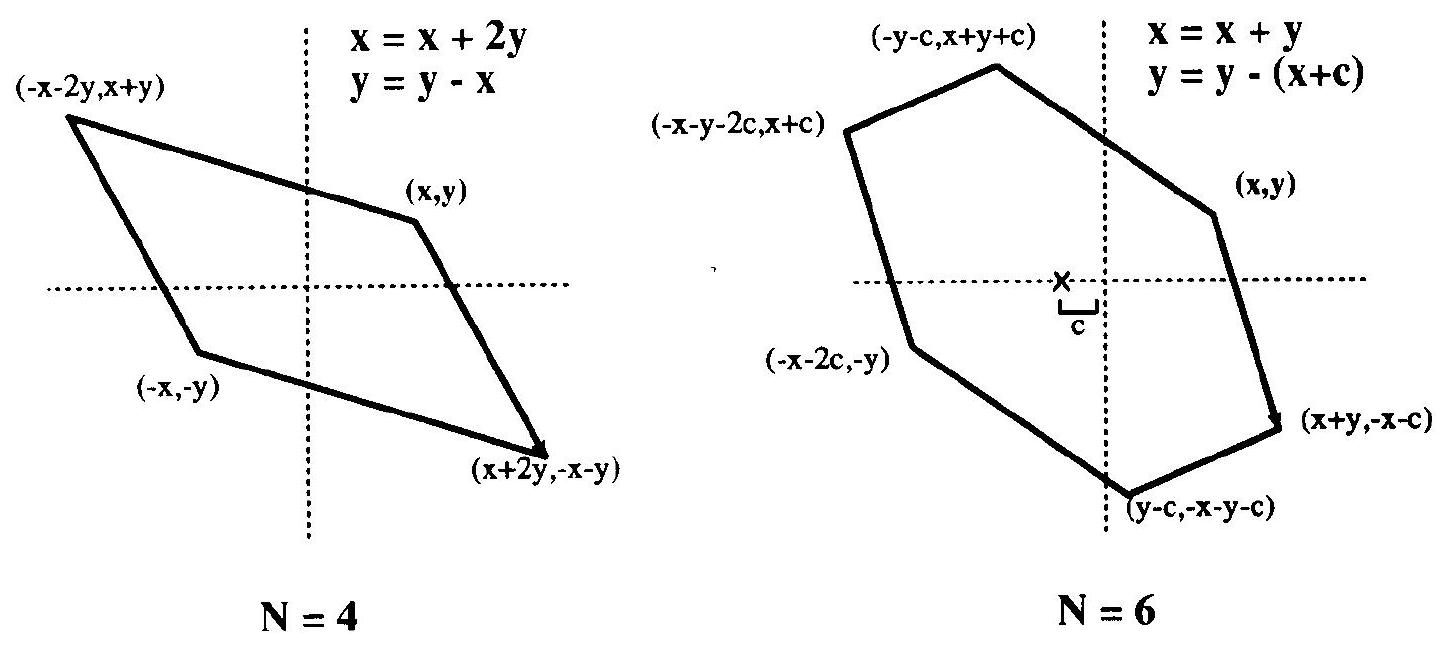
\includegraphics[max width=0.8\textwidth, center]{2022_11_30_0cbb01a33d99487fc27fg-104}
\caption{}
\end{figure}

我们对所有具有小乘数的三指令、三寄存器剪子进行了自动检查。没有发现新的$N$的解决方案,而且大多数形式没有明显的区别。双寄存器的 $N=3$的形式被用xor重写,导致(3.3)。$N=6$的双寄存器形式被认为可以容纳一个额外的常数,它抵消了$x$中的六边形,如图$1 b$所示,下面用代数法表示:

\begin{align}
\begin{aligned}
&a:=a+b; &a:\begin{bmatrix}
a &a+b & b+c &-a+2c & 2c-a-b &c-b 
\end{bmatrix}\\
&b:=b-a+c; &b:\begin{bmatrix}
b & c-a & c-a-b & -b & a-c & a+b-c
\end{bmatrix}
\end{aligned}
\tag{6.1}
\end{align}
当$\mathrm{c}=0$时,寄存器a中的值滞后于寄存器b中的值两步,提示存在一个(cos $t, \sin t)$生成器,除了$90^{\circ}$正交变成$120^{\circ}$相位偏移。通过$c \neq 0$,实现了一系列不同值的生成,达到了最初的目标。设置$\mathrm{c}=-1$允许使用逻辑补体- $(\mathrm{a}+1)$项的隐式形式(Paeth和Schilling, 1991),给出:

\begin{align}
\begin{aligned}
& a=b=1 ; \quad \textit { six-fold fixed-ualue cycle } \\
& \textbf { repeat } \\
& \qquad \mathrm{a}:=\mathrm{a}+\mathrm{b} ; \qquad \mathrm{a}:\left[\begin{array}{llllll}1 & 2 & 0 & -3 & -4 & -2\end{array}\right]\\
& \qquad \mathrm{b}:=\mathrm{b}+\textbf{not}(\mathrm{a}) ; \quad \mathrm{b}:\left[\begin{array}{llllll}1 & -2 & -3 & -1 & 2 & 3\end{array}\right]
\end{aligned}
\tag{6.2}
\end{align}
其中,c偏移量横向位移六边形的中心,消除了中心反转的对称性。这有助于实现不同的价值。对于$\mathrm{a}>0, \mathrm{~b}>0$和$2 \mathrm{c}>\mathrm{a}+\mathrm{b}$, $\mathrm{a}$中的序列始终为正。

\subsection*{$\mathbf{N=6}$ (触发)}
使用六重形式可以任意触发。上述算法的不同值允许并发1-in- $\mathrm{N}$触发器具有任何相位偏移。然而,带有非相邻触发器的2-in-N和3-in- $\mathrm{N}$形式存在更大的困难:它们可能不能通过用不等式替换相等测试来创建。这是图形凸性的结果:在几何术语中,像y $>4$这样的测试表示值的水平半空间。多边形与平面的交点将其分割为两个相邻顶点的不同边界集。目标是一个简单的触发器,它不需要像上面引用的Gem那样使用寄存器内位测试。

6个状态允许64个触发模式,其中第i个位置的“*”(“.”)表示第i个状态的触发器解除。互补模式的消除使这个数字减半。包含重复触发器的模式,如“***\textit{...”和“}*.*.*.”可以分解为超循环或子循环并被消除。左边是三个原型模式,分别设置了一个、两个或三个比特。测试使用(6.2)中的六倍旋转变量,隐含$(c=-1)$和起始值$a=b=0$:


\begin{align}
\begin{array}{rlrrrrrr}
\text { a: } & 0 & 0 & -1 & -2 & -2 & -1 \\
\text { b: } & 0 & -1 & -1 & 0 & +1 & +1 \\
\mathrm{a}=0 \text { AND b}= 0:&   * & \cdot & . & . & . & . \\
\mathrm{a}= 0: & * & . & * & . & . & . \\
\mathrm{a}=0 \text { OR } \mathrm{b}=0: & * & * & . & * & . & .
\end{array}
\tag{6.3}
\end{align}
\textbf{xor}的广泛使用提出了类似于在整数\textbf{mod}1上生成伪随机数(RPN)的方法(参见Morton, 1990)。传统的移位和携带测试逻辑硬件可以直接“连接”到三个\textbf{xor}寄存器指令,具有排列形式,给出

$$
\begin{aligned}
& \textbf { repeat } \quad \textit { cycle by seven }\\
& \qquad \mathrm{b}:=\mathrm{b} \textbf { xor } \mathrm{a} \text {; } \\
& \qquad \mathrm{c}:=\mathrm{c} \textbf { xor } \text{b;} \\
& \qquad \mathrm{a}:=\mathrm{a}\textbf { xor } \mathrm{b}
\end{aligned}
$$

这将产生如下所示的值表。

\begin{center}
\begin{tabular}{lll}
\hline
$\mathrm{A}$ & $\mathrm{B}$ & $\mathrm{C}$ \\
\hline
$\mathrm{a}$ & $\mathrm{b}$ & $\mathrm{c}$ \\
$\mathrm{a} \oplus \mathrm{b}$ & $\mathrm{b} \oplus \mathrm{c}$ & $\mathrm{a} \oplus \mathrm{b} \oplus \mathrm{c}$ \\
$\mathrm{a} \oplus \mathrm{c}$ & $\mathrm{a}$ & $\mathrm{b}$ \\
$\mathrm{c}$ & $\mathrm{a} \oplus \mathrm{b}$ & $\mathrm{b} \oplus \mathrm{c}$ \\
$\mathrm{a} \oplus \mathrm{b} \oplus \mathrm{c}$ & $\mathrm{a} \oplus \mathrm{c}$ & $\mathrm{a}$ \\
$\mathrm{b}$ & $\mathrm{c}$ & $\mathrm{a} \oplus \mathrm{b}$ \\
$\mathrm{b} \oplus \mathrm{c}$ & $\mathrm{a} \oplus \mathrm{b} \oplus \mathrm{c}$ & $\mathrm{a} \oplus \mathrm{c}$ \\
\hline
\end{tabular}
\end{center}
这里A列领先B两步,同样$B$领先$C$,但$C$领先A三步。每一列取三个变量中所有$\mathrm{N}-1$可能的\textbf{xor}排列,省略了禁止的零状态。这并不限制零元素的周期性生成,可以通过将$\{a, b, c\}$的任意(而不是全部)设为零,或者将两个寄存器中的初始值相等来形成,因为$\mathrm{M}$ \textbf{xor} $\mathrm{M}=0$。

使用四个寄存器$(r=4)$表示$2^{4}-1=15$状态。由于$r$是偶数,$\mathrm{N}$是因子$\left(2^{2}+1\right)\left(2^{2} -1\right)$的复合。这揭示了$\mathrm{N}=5$的子循环,将小$\mathrm{N}$的表舍入。然而,这种方法比旅法(5个变量,1个临时寄存器,6个分配)只显示了边际增益,因此没有进行研究。对于那些倾向于大$\mathrm{N}$的人,可以使用因子来组成更大的循环:相对素数长度的并发循环在若干步等于它们长度的乘积(GCM)后重新同步。

对于最后一个个位数值,$\mathrm{N}=9$仍然很困难,因为它既不是质数,也不是无平方的合数。$(11,13)$的下一个质数不属于$2^{\mathrm{m}}-1$梅森形式。根据费马定理,它们(和任何质数p)都是$2^{p-1}$的因数,这里$2^{10}-1$和$2^{12}-1$。由于这意味着寄存器的数量至少与\textbf{xor}方法的周期长度呈线性增长,因此brigade方法由于简单而获胜。尽管到目前为止所探索的所有方法的实际限制都是$\mathrm{N}<8$,但更奇特和更复杂的方法是可能的,并且可以通过暴力手段进行检查。其中之一如下所示。

\subsection*{$\bf{
N=24
}$}

作为最后一个例子,代码

$$
\begin{aligned}
&\textbf { register } a=4 ; \\
&\textbf { register } b=3 ; \\
&\textbf { repeat }\\
&\qquad \mathrm{a}:=\mathrm{a}-\mathrm{b};\\
&\qquad \mathrm{a}:=\mathrm{a} \textbf{ bit-and } 15; \textit{explicit limit on register a}\\
&\qquad \mathrm{b}:=\mathrm{b} \textbf{ xor } \mathrm{a} ;
\end{aligned}
$$
提供了一种循环模24的方法。将寄存器$a$的域限制为16个值必然会引入值的多样性。所选的初始值将$a$和$b$限制在域[1..]并进一步保证它们永远不会同时相等。

这段代码的价值是分别使用条件测试$(b=1)、(a=4)、(b=7)$和$(b=12)$形成并行的24:1、12:1、8:1和6:1的速率除法。这些测试被选择,因此在任何步骤中最多一个为真,通过将$\{1,2,3,4\}$ -in-24测试通过触发位的ring组合,允许速率乘法(最多10-in-24)。注意,只有3 / 24的比率显示出轻微的不均匀性:

\begin{table}
%\tiny
%\resizebox{\textwidth}{10mm}{
\setlength{\tabcolsep}{1mm}{%控制单元格前后间距间接控制单元格宽度
\begin{tabular}{ccccccccccccccccccccccccc}
a :& 1& 15& 2& 3& 7& 12& 5& 3& 2& 15& 3& 4& 9& 7& 2& 11& 15& 12& 13& 1& 12& 7& 11& 4  \\ 
b :& 2& 13& 15& 12& 11& 7& 2& 1& 3& 12& 15& 11& 2& 5& 7& 12& 3& 15& 2& 9& 11& 12& 7& 3\\
\hline 
b=1 :& * & • & • & • & • & • & • & • & • & • & • & • & • & • & • & • & • & • & • & • & • & • & • \\ 
a=4 :& • & • & • & • & • & • & • & • & • & • & • & • & * & • & • & • & • & • & • & • & • & • & &* \\ 
b=7 :& • & • & • & • & • & * & • & • & • & • & • & • & • & • & * & • & • & • & • & • & • & • & * \\ 
b=12 :& • & • & • & * & • & • & • & • & • & * & • & • & • & • & • & * & • & • & • & • & • & * & • \\
\end{tabular} 
}
\end{table}
\subsection*{总结}
给出了循环生成任意值和布尔状态的方法。对$N=\{2,3,4,6,7\}$的情况进行了详细的处理。附录中提供的大量c代码变体为图形程序员的技巧包提供了一组有用的补充。

See also G1, 436.

\newpage
\section{一个通用的像素选择机制}
\begin{center}
\small{
Alan W. Paeth\\
NeuralWare Incorporated\\
Pittsburgh, Pennsylvania}
\end{center}

反转帧缓冲区像素的颜色是突出显示区域的常用方法。一个有用的反转函数提供了视觉上不同的颜色对。在较新的硬件上,查找表(映射像素的外观)是通过窗口输入的,引入了空间依赖性。这给“最佳”函数的设计带来了负担。这个宝石提供了一个简单的先验解决方案,可以保证视觉上不同的颜色对,尽管算法仍然不知道它们的最终外观。典型的用途是创建屏幕范围、窗口不变的工具,例如用于显示“快照”的系统游标或选择矩形。

一个有用的反求函数$F$在像素$p$上满足两个代数条件:$F(F(p))=p$和$F(p) \mu$ p。第一个条件保证函数是它自己的逆函数。第二个关键是保证任何颜色对中的两个元素“不几乎相等”,使它们在视觉上不同。对于一位像素,互补(位切换)是明显的解决方案。在更高的精度下,所有位的(ones)补变成了一个算术运算:$F(p)=\operatorname{not}(p)=-1-p$在2的补运算下(Paeth, 1991)。对于$0 \leq c<1$,这已经被推广(Newman和Sproull, 1979)为$F_{c}(p)=\operatorname{frac}(c-p)$。这不能满足第二个条件:对于参数c,值c/ 2的像素映射到它自己。几何上,单位区间已经显示(通过c),并映射到原始区间,从而引入一个静止点。

在调色板系统中使用的解决方案(Higgins和Booth, 1986)回到了逻辑运算作。给定一个二进制整数,它定义了沿区间的离散位置,仅最上面的位的位互补交换区间的上下半部分,而没有任何镜像。任何颜色对中的像素现在都被间隔距离的一半取代,以保证不同的颜色。对于颜色映射的像素(作为索引),一对中的元素在映射函数的域中被移除得很远,如果颜色映射定义了单调函数,则产生的颜色在范围内也被移除——这是一种常见的情况。某些非线性非笛卡尔色图(Paeth, 1991)在这个函数下也能很好地工作,并支持简单的几何解释。

现在可以通过做一些简单的假设来构造泛型函数。典型帧缓冲器上单色通道的像素精度为1位、4位或8位。操作
$$
\text { \textbf{macro} bwpixflip }(\mathrm{x}) \quad \mathrm{x}:=\mathrm{x} \textbf{ bit-xor } 133 \qquad \textit { hex  85}
$$
在不知道使用精度的情况下,对最上面的位进行补位。当底层像素精度较低时,切换高阶位无关紧要,或者被硬件写掩码的动作压制。相反,在高精度上的操作,像素将补充额外的低精度位,但这些被充分去除会产生很大的后果。

对于RGB像素,十六进制85的三个副本确保在三个相邻通道上操作。这还在第12位引入了一个切换,在硬件上提供了扩展的单色精度或颜色表索引。通用的颜色反转函数是
$$
\text { \textbf{macro} pixelflip(x) } \quad \mathrm{x}:=\mathrm{x} \textbf { bit-xor } 8750469 \qquad\textit { hex  858585}
$$
操作的三次使用将沿着每个颜色轴交换一半的单位间隔。从几何上看,这表示在单位颜色立方体中围绕中层灰色中心点$\left(\frac{1}{2},\frac{1}{2},\frac{1}{2}\right)$的八个子立方体的变换。在非魔方的方式下,每个立方体的朝向被保留(图2.6.1a)。在第一性原理“xor - 1”的情况下(未显示),八个立方体的附加中心反转反转了整个固体,并且在中间灰色位置重新引入了不希望出现的静止点。

\begin{figure}[htbp]
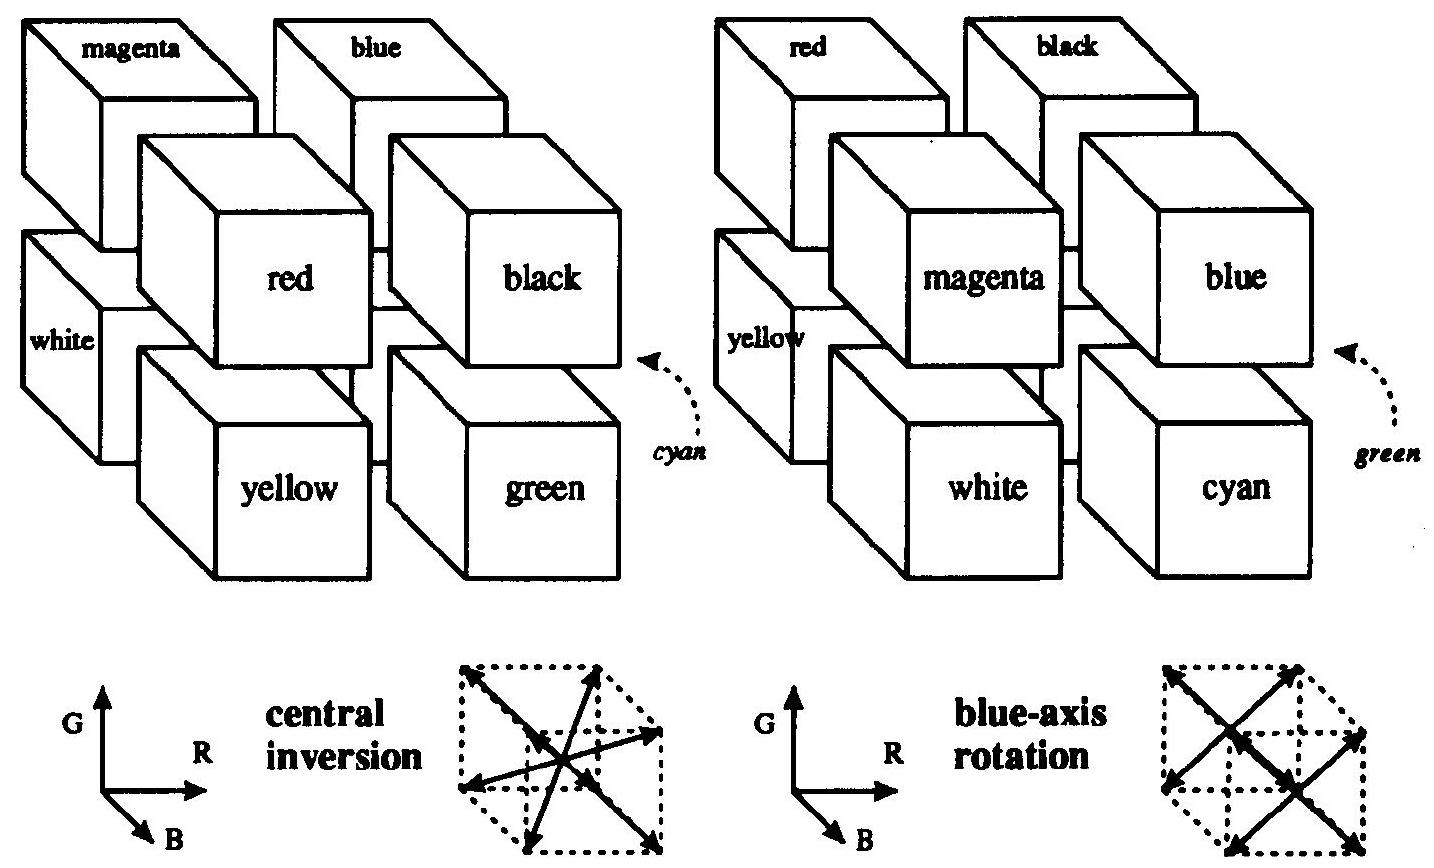
\includegraphics[max width=\textwidth]{2022_11_30_0cbb01a33d99487fc27fg-111}
\caption{•}
\end{figure}

最后,不补充蓝色通道通常是有利的。当蓝色占据最上面的像素位(如Adage/ Ikonas或SGI/ Iris)时,定义红色和绿色通道的下16位的互补仍然发生;所有单色和查找情况(像素精度从不超过16位)也隐含地涵盖。另一个通用宏是
$$
\text { \textbf{macro} pixelflip2(x) } \quad \mathrm{x}:=\mathrm{x} \textbf { bit-xor } 34181 \textit { hex  8585}
$$
对于24位颜色,保留蓝色意味着子立方体不再通过中心反转交换(图la),而是以“摩天轮”方式围绕蓝色轴旋转半圈(lb)。这就产生了一对对立的颜色(红、绿),人类的视觉系统对它们的反应非常灵敏,再加上一对(蓝、白)、(青色、品红)和(黄、黑)。备用宏支持在反转中使用短的16位整数。

See also G1, 215; G1, 219; G1, 233; G1, 249.

\newpage
\section{经扭曲的非均匀随机点集}
\begin{center}
\small{
Peter Shirley\\
Indiana University\\
Bloomington, Indiana}
\end{center}

我们经常希望在单位正方形上生成随机或伪随机点集,用于分布射线跟踪等应用。有几种方法可以做到这一点,例如抖动和泊松盘采样。这些方法给出了一组在单位正方形上合理分布的$\mathrm{N}$点:$\left(u_{1}, v_{1}\right)$到$\left(u_{N}, v_{N}\right)$。

有时,我们的采样空间可能不是方形的(例如,圆形透镜)或可能不是均匀的(例如,以像素为中心的滤波函数)。如果我们能写一个数学变换,将我们的等分布点$\left(\mathrm{u}_{\mathrm{i}}, \mathrm{v}_{\mathrm{i}}\right)$作为输入,并以期望的密度在期望的采样空间中输出一组点,那就太好了。例如,要对一个相机镜头进行采样,变换将取$\left(\mathrm{u}_{\mathrm{i}}, \mathrm{v}_{\mathrm{i}}\right)$并输出$\left(r_{i}, \theta_{i}\right)$,使新点在镜头的圆盘上近似均匀分布。

结果表明,这种变换函数在蒙特卡罗积分领域是众所周知的。表2.7.1给出了对计算机图形学有用的几种转换的表格。本文其余部分将讨论生成这种转换的方法。请注意,其中一些转换可以简化为简单密度。例如,要生成余弦分布的方向,使用Phong密度和$\mathrm{n}=1$。要在单位半球上生成点,使用单位球密度上的扇区,带$\theta_{1'}=0, \theta_{2}=\pi / 2, \varphi_{1}=0$和$\varphi_{2}=\pi$。

对于蒙特卡罗方法,我们必须经常根据某个概率密度函数生成随机点,或根据某个方向概率密度生成随机射线。在本节中,将描述一种一维和二维随机变量的方法。本文的讨论紧跟Shreider(1966)的讨论。

\begin{table}[htbp]
\small{\caption{(符号$u, v$和$w$表示范围超过[0,1]的均匀分布随机变量的实例。)}}
\centering
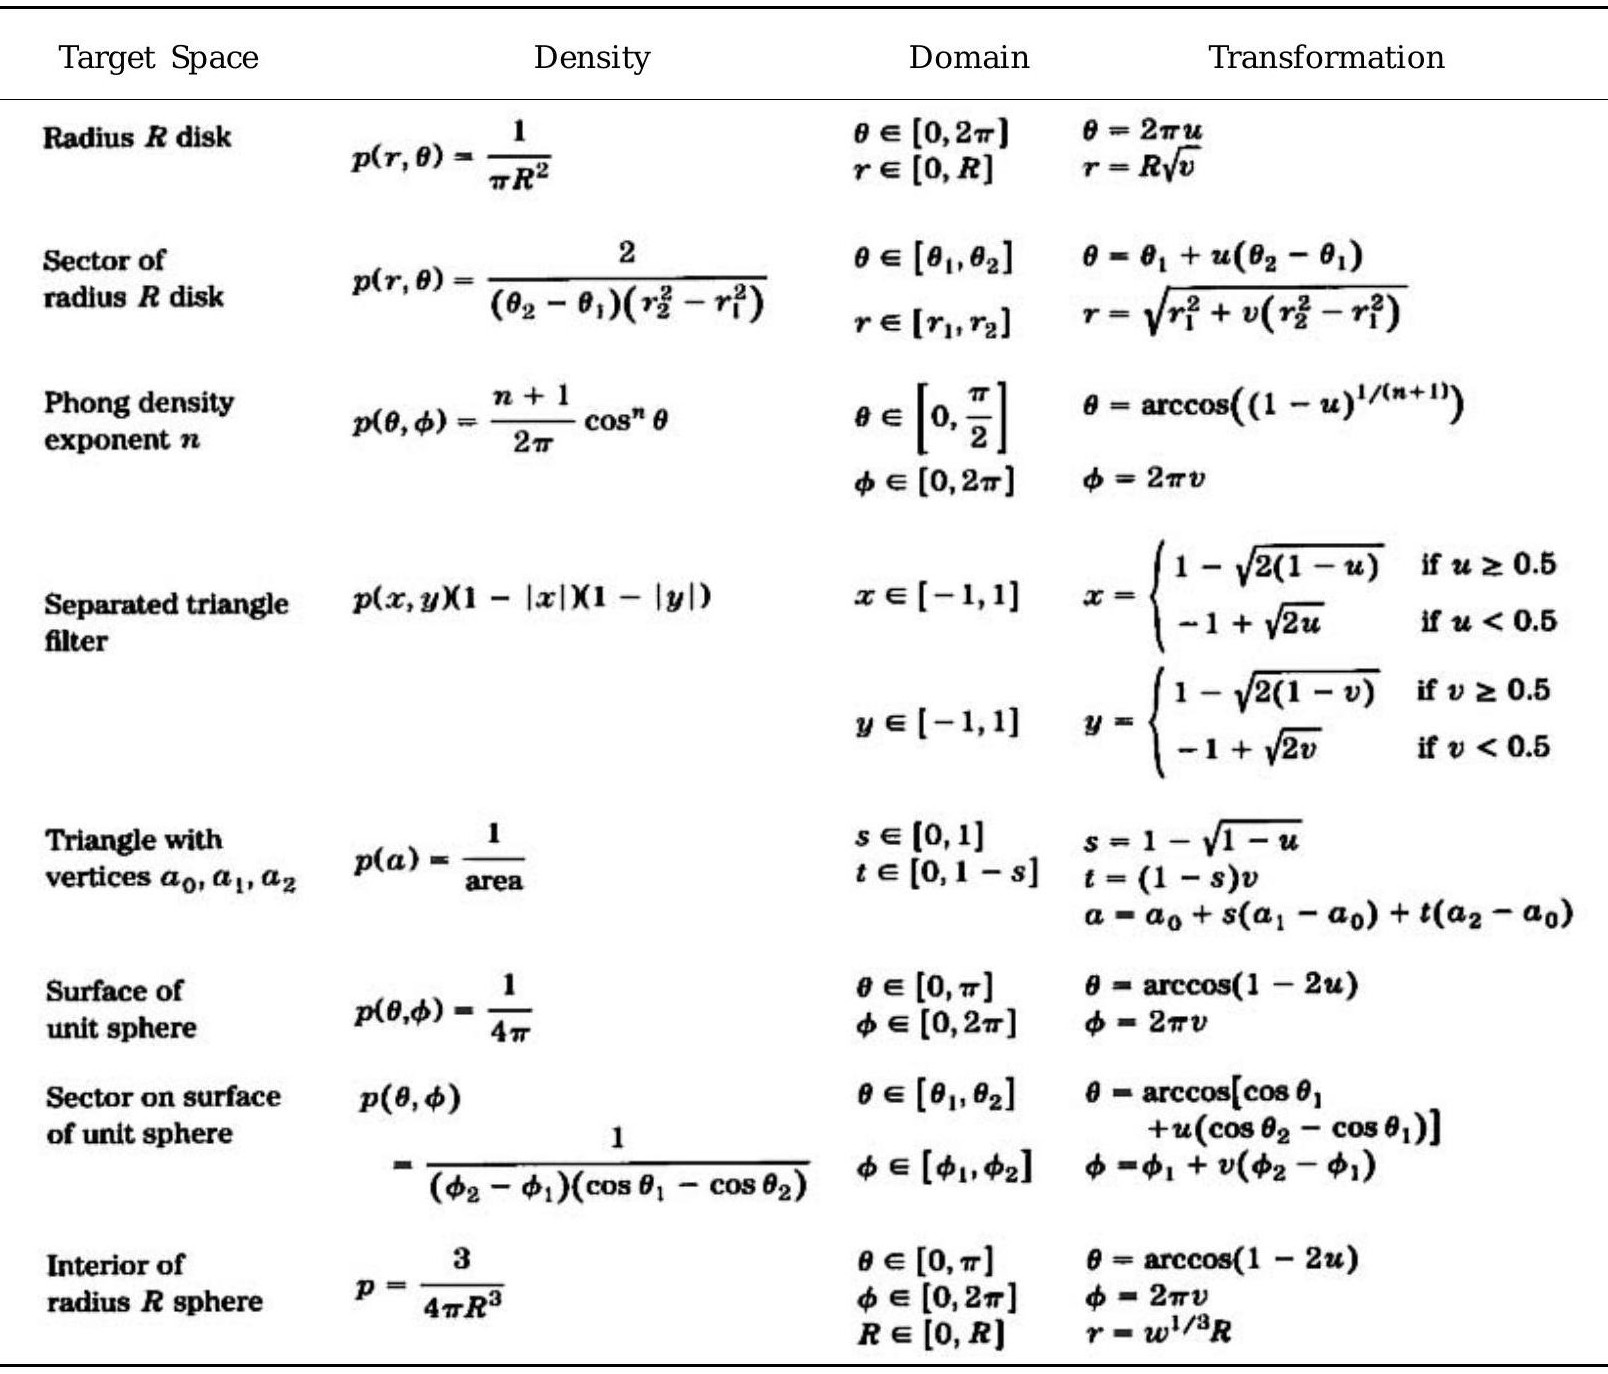
\includegraphics[totalheight=4in]{2022_11_30_0cbb01a33d99487fc27fg-113}
\end{table}

如果密度是在区间$\mathrm{x} \in[\mathrm{a}, \mathrm{b}]$上定义的一维$\mathrm{f}(\mathrm{x})$,那么我们可以从一组均匀随机数$\xi_{\mathrm{i}}$中生成具有密度$\mathrm{f}$的随机数$\alpha_{\mathrm{i}}$,其中$\xi_{\mathrm{i}} \in[0,1]$。为此,我们需要概率分布函数$\mathrm{F}(\mathrm{x})$:
\begin{align}
F(x)=\int_{a} f\left(x^{\prime}\right) d \mu\left(x^{\prime}\right)
\end{align}
要得到$\alpha_{\mathrm{i}}$,只需转换$\xi_{\mathrm{i}}$:
$$
\alpha_{\mathrm{i}}=\mathrm{F}^{-1}\left(\mathrm{x}_{\mathrm{i}}\right) \text {, }
$$
其中$\mathrm{F}^{-1}$是$\mathrm{F}$的倒数。如果$\mathrm{F}$不是解析可逆的,那么数值方法就足够了,因为所有有效的概率分布函数都存在一个逆。

如果我们有一个二维密度$(\mathrm{x}, \mathrm{y})$定义在[a, b: c, d]上,那么我们需要二维分布函数:
\begin{align}
F(x, y)=\int_{c}^{y} \int_{a}^{x} f\left(x^{\prime}, y^{\prime}\right) d \mu\left(x^{\prime}, y^{\prime}\right) .
\end{align}
我们首先使用边缘分布$\mathrm{F}(\mathrm{x}, \mathrm{d})$选择$x_i$,然后根据$F\left(x_{i}, y\right) / F\left(x_{i}, d\right)$选择$y_{i}$。如果$F(x, y)$是可分离的(可表示为$g(\mathrm{x}) \mathrm{h}(\mathrm{y}))$,则一维技术可用于每个维度。

例如,为了选择反射射线方向进行分区计算或分布式射线跟踪,我们可以将问题看作是在单位球或半球上选择点(因为每个射线方向可以表示为球上的一个点)。例如,假设我们想要根据密度来选择射线
\begin{align}
p(\theta, \phi)=\frac{n+1}{2 \pi} \cos ^{n} \theta,
\end{align}
其中$\mathrm{n}$是一个Phong-like指数指数;$\theta$是与曲面法线的夹角,$\theta \in[0, \pi / 2]$(在上半球);$\phi$是方位角$(\phi \in[0,2 \pi])$。分布函数为
\begin{align}
P(\theta, \phi)=\int_{0}^{\varphi} \int_{0}^{\theta} \mathrm{p}\left(\theta, \varphi^{\prime}\right) \sin \theta' \mathrm{d} \theta' \mathrm{d} \phi^{\prime} .
\end{align}
$\sin \theta$项的产生是因为$\mathrm{d} \omega=\sin \theta \mathrm{d} \theta \mathrm{d} \varphi$在球面上。当发现边缘密度时,$p$(如预期的那样)是可分离的,我们发现$\left(r_{1}, r_{2}\right)$均匀随机数可以被变换到一个方向
\begin{align}
(\theta, \phi)=\left(\arccos \left(\left(1-r_{1}\right)^{1 /(n+1)}\right), 2 \pi r_{2}\right) .
\end{align}
通常,我们希望一个方向$(\theta, \phi)$对是关于某个单位向量$\mathrm{y}$的(而不是$\mathrm{z}$轴)。要做到这一点,我们可以首先将角度转换为单位向量$a$:
$$
a=(\cos \phi \sin \theta, \sin \phi \sin \theta, \cos \theta) .
$$
然后,我们可以将$a$转换为关于$\psi$的$a'$,方法是将a乘以旋转矩阵$\mathrm{R}\left(a'=Ra\right.)$ 。这个旋转矩阵写起来很简单:
$$
R=\begin{bmatrix}
u_{x} & v_{x} & w_{x} \\
u_{y} & v_{y} & w_{y} \\
u_{z} & v_{z} & w_{z}
\end{bmatrix},
$$
其中$u=\left(u_{x}, u_{y}, u_{z}\right), v=\left(v_{x}, v_{y}, v_{z}\right), w=\left(w_{x^{\prime}} w_{y^{\prime}}, w_{z}\right)$,形成一个基(一个单位向量的标准正交集,其中$u=v\times w, v=w\times u$, 和 $w=u\times v$),形成一个约束$w$与$\psi$对齐的基。:
$$
\mathrm{w}=\frac{\psi}{|\psi|} .
$$
为了得到$u$和$v$,我们需要找到一个与$w$不相交的向量$t$。要做到这一点,只需将$t$设为$w$,并将$t$的最小幅度分量改为1。$u$和$v$很容易得到。
$$
\begin{aligned}
&u=\frac{t \times w}{|t \times w|}, \\
&v=w\times u .
\end{aligned}
$$
这个技术系列对许多采样应用非常有用。不幸的是,一些抽样空间(如十二面体的表面)并不能自然地使用本宝石中的方法来处理。这时就需要特殊的目的,或者作为最后的手段,需要拒绝技术。



See also G1, 438.

\newpage
\section{四维及四维外的叉乘}
\begin{center}
\small{
Ronald N. Goldman\\
Rice University\\
Houston, Texas}
\end{center}

\subsection*{介绍}
叉积是上帝赐予人类的伟大礼物之一。它在数学、物理、工程,当然还有计算机图形学方面有很多应用。法向量、旋转、旋度、角动量、扭矩和磁场都利用叉乘。

在三维空间中给定两个线性无关的向量$u$和$v$,它们的叉积是垂直于$u$和$v$平面的向量$u \times v$,根据右手规则定向,其长度等于$|u||v| \sin \Theta$,其中$\Theta$是$u$和$v$之间的角度。在直角坐标系中中,叉积可以通过简单的行列式计算出来
$$
u \times v=\left|\begin{array}{ccc}
\mathbf{i} & \mathbf{j} & \mathbf{k} \\
u_{1} & u_{2} & u_{3} \\
v_{1} & v_{2} & v_{3}
\end{array}\right| .
$$
相当于,
$$
u \times v=\left(u_{2} v_{3}-u_{3} v_{2}, u_{3} v_{1}-u_{1} v_{3}, u_{1} v_{2}-u_{2} v_{1}\right) \text {. }
$$
乍一看,叉乘似乎是三维的产物。在三维空间中,由两个向量决定的平面法线方向是唯一的,但在四维空间中,有一整个平面的向量都是与任何给定平面法向的。因此,如何在四维空间中定义两个向量的叉乘是不清楚的。那么在四维及四维以外的空间里叉乘的类似物是什么呢?这个宝石的目标就是回答这个问题。

\subsection*{张量积}
有一种看待叉乘的方法比标准定义更有指导意义而且很容易推广到四维或四维以上。为了理解这种方法,我们需要从两个向量的张量积的概念开始。

张量积$u \otimes v$被定义为方阵
$$
u \otimes v=u^t * v,
$$
其中上标$t$表示转置,$*$表示矩阵乘法。同样,
$$
(u \otimes v)_{i j}=\left(u_{i}, v_{j}\right) .
$$
注意,对于任意向量w,
$$
\mathrm{w}(\mathrm{u} \otimes \mathrm{v})=(\mathrm{w} \cdot \mathrm{u}) \mathrm{v} .
$$
因此,张量积与点积密切相关。

像点积一样,张量积对于任意维的两个向量都有意义。的确,张量积具有点积的许多代数性质。然而,与点积不同,张量积不是可交换的。也就是说,总的来说,

$$
u \otimes v \neq v \otimes u \quad \text { 因为 } u_{i} v_{j} \neq u_{j} v_{i}
$$
Goldman(1990,1991)给出了两个向量张量积在计算机图形学中的应用。

\subsection*{楔积}
两个向量$u$和$v$的楔积测量了它们张量积的不可交换性。因此,楔积$u \wedge v$是由定义的方阵
$$
u \wedge v=u \otimes v-v \otimes u .
$$
相当于,
$$
(u \wedge v)_{i j}=\left(u_{i} v_{j}-u_{j} v_{i}\right) .
$$
像张量积一样,楔形积定义为任意维的两个向量。还要注意,楔积和叉积有许多相同的性质。例如,从楔积定义为两个张量积之差可以很容易地直接验证:
$$
\begin{aligned}
& u \wedge u=0, \\
& u \wedge v=-v \wedge u &\text{(反交换律)},\\
& u *(v \wedge w) \neq(u \wedge v) * w^{t} &\text{(非结合律)},\\
& u \wedge cv=c(u \wedge v)=(cu) \wedge v, & \\
& u \wedge(v+w)=u \wedge v+u \wedge w &\text{(分配律)},\\
& u *(v \wedge w)+v *(w \wedge u)+w *(u \wedge v)=0 &\text{(Jacobi恒等式)},\\
& r *(u \wedge v) * s^{t}=(r \cdot u)(s \cdot v)-(r \cdot v)(\mathrm{s} \cdot u) &\text{(Lagrange恒等式)}.
\end{aligned}
$$

楔积与叉积还具有其他一些重要的性质。叉乘的定义特征由公式得到
$$
\begin{gathered}
u \cdot(u \times v)=v \cdot(u \times v)=0, \\
|u \times v|=|u|^{2}|v|^{2} \sin ^{2} \Theta .
\end{gathered}
$$
根据Lagrange恒等式,楔积满足类似恒等式:
$$
\begin{aligned}
&u *(u \wedge v) * u^{t}=\mathrm{v} *(u \wedge v) * v^{t}=0, \\
&u *(u \wedge v) * v^{t}=(u \cdot u)(v \cdot v)-(u \cdot v)^{2}=\left|u\right|^{2}\left| v\right|^{2} \sin ^{2} \Theta
\end{aligned}
$$
通过定义矩阵$M$的范数为下式,可以生成最后一个单位的变体
$$
|M|^{2}=\frac{1}{2}\left\lbrace \sum_{i j}\left(M_{i j}\right)^{2} \right\rbrace .
$$
通过直接计算很容易验证
$$
|u \wedge v|^{2}=(u \cdot u)(v \cdot v)-(u \cdot v)^{2}=|u|^{2}|v|^{2} \sin ^{2} \Theta .
$$
另外,叉乘恒等式
$$
(u \times v) \times w=(w \cdot u) v-(w \cdot v) u
$$
有楔积的类似物
%has the wedge product analogue
\begin{align}
w \cdot(u \wedge v)=(w \cdot u) v-(w \cdot v) u .
\label{eq:2.8.1}
\end{align}
叉乘可以用来测试垂直于$u$和$v$平面的向量,因为
$$
w \times(u \times v)=0 \Leftrightarrow \mathrm{w} \perp u, v .
$$
类似地,楔形积识别垂直于由$u$和$v$决定的平面的向量,因为通过公式\ref{eq:2.8.1},
$$
w *(u \wedge v)=0 \Leftrightarrow(w \cdot u)=(w \cdot v)=0 \Leftrightarrow w \perp u, v .
$$
此外,在三维空间中,
$$
u \wedge v=\left|\begin{array}{ccc}
0 & u_{1} v_{2}-u_{2} v_{1} & u_{1} v_{3}-u_{3} v_{1} \\
u_{2} v_{1}-u_{1} v_{2} & 0 & u_{2} v_{3}-u_{3} v_{2} \\
u_{3} v_{1}-u_{1} v_{3} & u_{3} v_{2}-u_{2} v_{3} & 0
\end{array}\right|
$$
因此,在三维空间中,楔积矩阵$u \wedge v$的分量,与叉乘向量$u \times v$的分量,在符号上是相同的。这个观察解释了为什么楔积和叉积共享如此多的代数性质。

在三维空间中我们非常幸运。矩阵$u \wedge v$是反对称的,所以到符号为止,它只有三个唯一的分量。这个性质允许我们用向量$u \times v$来识别矩阵$u \wedge v$。然而,对于向量$u \times v$,有一些非常特殊的东西。如果$u$和$v$是正交的单位向量,则向量$u, v, u \times v$形成一个右手坐标系。但如果$\mathrm{M}$是映射$u, v$平面上向量的线性变换,则$\{u \cdot M, v \cdot M,(u \times v) \cdot M\}=\{u, v,-u \times v\}$构成一个左手坐标系。因此,$(u \cdot M) \times (v \cdot M) \neq(u \times v) \cdot M$,因此$u \times v$并不真正转换为一个向量。这个反常现象应该提醒我们,叉乘并不是一个真正的向量。事实上,叉乘变换更像张量而不是向量。


In higher dimensions we are not nearly so lucky. For example, in four dimensions the antisymmetric matrix $u \wedge v$ has, up to sign, six, not four, distinct entries. Thus, the matrix $u \wedge v$ cannot be identified with a four-dimensional vector. In $\mathrm{n}$ dimensions, the antisymmetric matrix $\mathrm{u} \wedge \mathrm{v}$ has $n(n-1) / 2$ unique entries. But $n(n-1) / 2 \neq n$ unless $n=0,3$. Thus, only in three dimensions can we identify the wedge product of two vectors with a vector of the same dimension. In general, the wedge product is an antisymmetric 2-tensor. This antisymmetric tensor shares many of the important algebraic properties of the cross product, and thus it is a natural generalization of the cross product to four dimensions and beyond.

\subsection*{Acknowledgment}
I would like to thank Joe Warren for pointing out that the formula for the length of the cross product $u \times v$ has a direct analogue in the formula for the norm of the wedge product $u \wedge v$.

\newpage
\begin{center}
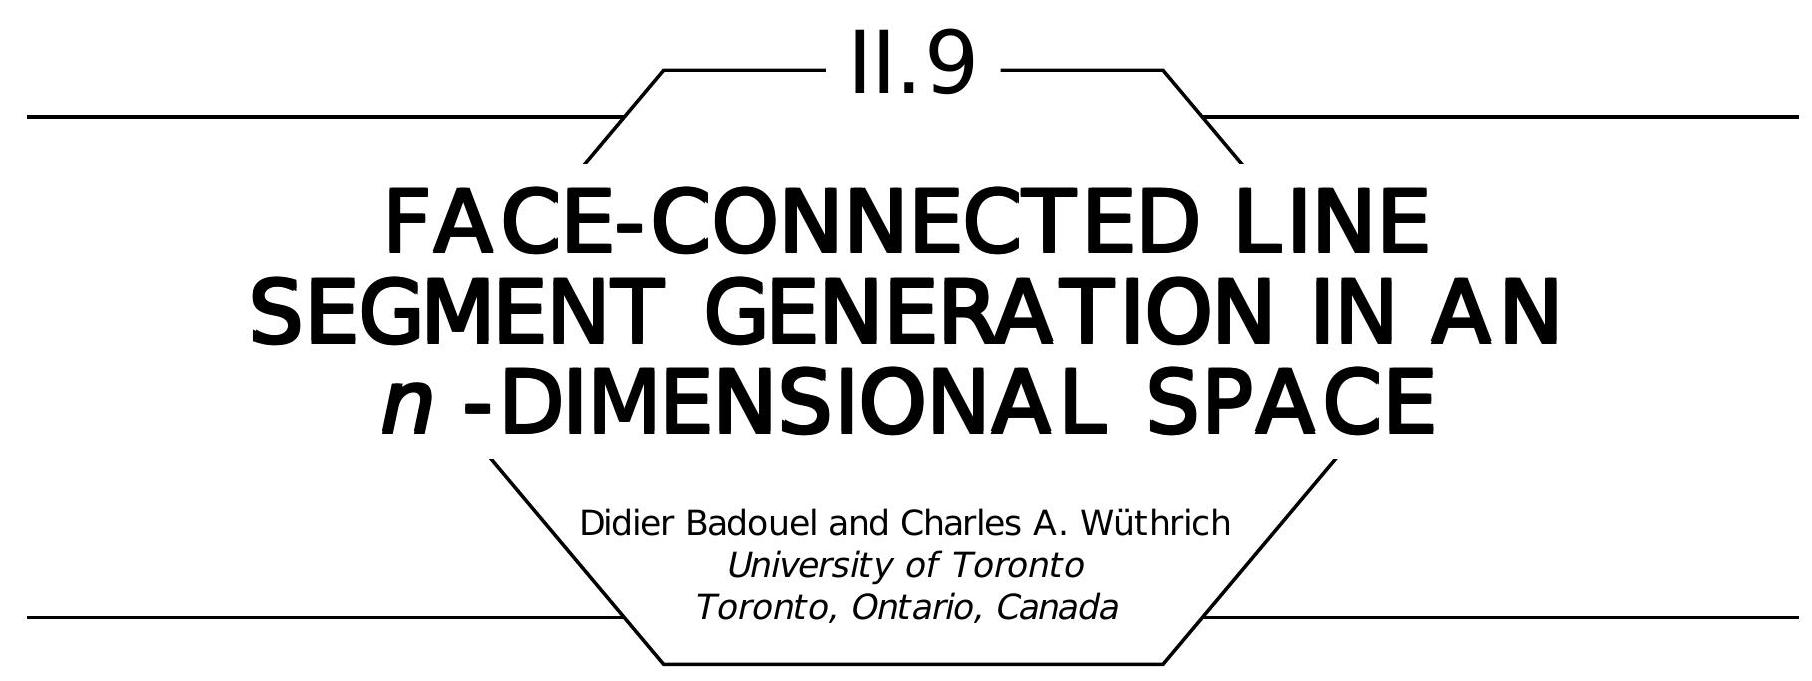
\includegraphics[max width=\textwidth]{2022_11_30_0cbb01a33d99487fc27fg-121}
\end{center}

In the early days of Computer Graphics, straight line rasterization was developed to render segments onto the raster plane. Later, three-dimensional segment discretization had to be developed to keep track of the path of a ray in the object space. These algorithms generate a connected sequence that represents the segment in the discrete space; moreover, they define a path in which the directions are uniformly distributed. An extension to higher-dimensional spaces is suited for applications ranging from line generation in a time-space coordinate system to the incremental generation of a discrete simultaneous linear interpolation of any number of variables.

This gem presents an algorithm that generates a face-connected line segment in discrete n-dimensional spaces. In two dimensions, the algorithm introduced below coincides with any classical 4-connected straight line drawing algorithm. Among all discrete segments joining two points, this algorithm produces one in which the directions are uniformly distributed. A definition of uniform distribution is given below.

Consider an n-dimensional lattice, or hyperlattice, i.e., the set of all points $\mathrm{P}=\left(\mathrm{p}_{0}, \mathrm{p}_{1}, \ldots, \mathrm{p}_{\mathrm{n}-1}\right)$ of $\mathbf{Z}^{\mathrm{n}}$ : Neighbourhood relations can be defined between the Voronoi hypervroxel associated with each point of the hyperlattice. In fact, only voxels having a hyperface in common, i.e., corresponding to hyperlattice points having $\mathrm{n}-1$ coordinates in common, will be considered here as neighbours. In a two-dimensional lattice, such neighbourhood relation is the well-known 4 -connection, while in the three-dimensional space it leads to 6-connection. The neighbourhood relations among the hyperlattice points introduce a rasterization proce- dure for curves into the hyperlattice: A rasterization of a curve is in fact a path of neighbouring lattice points.

Consider two hyperlattice points $P=\left(p_{0^{\prime}}, p_{1}, \ldots, p_{n-1}\right)$ and $Q=$ $\left(q_{0^{\prime}} q_{1}, \ldots, q_{n-1}\right)$. Let $n_{i}=\left|q_{i}-p_{i}\right|$ Then a face-connected shortest path between $\mathrm{P}$ and $\mathrm{Q}$ requires $\mathrm{m}=\sum \mathrm{n}_{\mathrm{i}}$ steps. The hyperline points are the points of coordinates $x_{i}=\left(q_{i}-p_{i}\right) t+p_{i}$, with $t \in[0,1]$. The parameter $t$ introduces an ordering on the points of the straight line. Consider the straight line points $P_{i, h_{1}}$ obtained for $t=h_{i} / n_{i}$, where $h_{j}=1, \ldots, n_{i}$, and order them in increasing order of their corresponding parameter value. Whenever an ambiguity occurs, and two parameter values $h_{\mathrm{j}} / \mathrm{n}_{\mathrm{i}}$ and $h_{\mathrm{j}} / \mathrm{n}_{\mathrm{j}}$ coincide, an arbitrary order has to be chosen. In other words, the segment $\mathrm{PQ}$ is subdivided into $\mathrm{n}_{\mathrm{i}}$ parts for each dimension i, and the points obtained on the straight line segment are ordered by increasing values of the parameter t. When two subdivision points coincide, the one corresponding to the smaller dimension is considered to precede the other one.

The resulting set is a finite ordered set of the segment points $P_{i, h_{i}}$, which can be renamed as $A_{0^{\prime}} A_{1}, \ldots, A_{m-1}$ Consider the finite path built by taking the sequence of directions $\left\{a_{k}\right)_{k=0, \ldots, m-1}$, such that each direction $a_{k}$ corresponds to the point $A_{k}=P_{a_{k}, 1}$, for some l. Such a path is said to be uniformly distributed with respect to the directions that constitute it. It is clear that in such a path the occurrences of the different directions that have to appear in it are as evenly spaced as possible in the chain. Moreover, if we follow the previously defined path from the point $\mathrm{P}$, the point $\mathrm{Q}$ shall be reached.

Whenever the hyperface-connected rasterization onto the n-dimensional hyperlattice of a straight line segment joining two hyperlattice points is computed, the result is a hyperface-connected path joining the two points. This path is uniformly distributed among all directions. A simplified version of the routing algorithm can be therefore summarized as follows. For each direction $i$, an integer counter $d_{i}$ is used. In order to generate the straight line between the two points $P$ and $Q$, the values of $\mathrm{n}_{\mathrm{i}}$ are computed. Their least common multiple $\mathrm{l}=\mathrm{LCM}\left(\mathrm{n}_{\mathrm{i}}\right)$ is evaluated, ${ }^{1}$ and the values of $\mathrm{n}_{\mathrm{i}}^{\prime \prime}=1 / \mathrm{n}_{\mathrm{i}}$ are computed. To obtain only integer

${ }^{1}$ In fact, either a low-complexity method in $\mathrm{O}(\mathrm{n} \log \mathrm{k})$ based on a table lookup or a simple common multiple can be used here. computations, the values of $n_{i}^{\prime}=2 n^{\prime \prime}$ are used. The cells $d_{i}$ are initialized to the value $n_{i}^{\prime} / 2$. This initialization has to be made, otherwise the path generated corresponds to another rasterization scheme. At each step, $\mathrm{n}_{\mathrm{i}}^{\prime}$ is added to the di with the smallest value, and the ith signed direction is generated. The generation procedure is repeated until all $d_{i}$ have reached the value $2 l+n_{i}^{\prime \prime}$. which is equivalent to $\forall i, d_{i} \geq 2 l$.\\




\end{CJK}